\label{sec:pac}
% \rnote{For this section, you should first define PAC-Bayes bound and explain the role of prior and posterior. Then you should say what posterior \cite{dziugaite2017computing} optimize over and explain how our posterior is different. After that skip all the details about calculation and directly show the results (the table, the figures might also belong to appendix). This shouldn't be a very long section.}
%\cnote{We need to briefly explain the PAC-Bayes bound in \citet{dziugaite2017computing}, e.g., what is SNN, what does the bound look like, what's prior/posterior.
%Given a model parameterized with $\vtheta$ and an input-label pair $(\vx,\vy)\in\R^d\times \R^c$, the classification error of $\vtheta$ over the input sample $\vx$ is $\breve{l}(\vtheta, \vx) := \1[\argmax f_\vtheta(\vx) = \argmax\vy].$ With the underlying data distribution $D$ and training set $S$ i.i.d. sampled from $D$, we define
%$e(\vtheta):=\E_{(\vx, \vy)\sim D}[\breve{l}(\vtheta,\vx)], \hat{e}(\vtheta):=\frac{1}{N}\sum_{i=1}^N[\breve{l}(\vtheta,\vx_i)]$
%as the expected and empirical classification error of $\vtheta$, respectively.
%Let the measurable hypothesis space of parameters be $\gH:= \R^P$.
%\znote{measurability is stated for KL to be generally well-defined, do we need to define $P$ and $Q$ as probability measure as well?}
%For any probabilistic measure $P$ in $\gH$, let $e(P) = \E_{\vtheta\sim P}e(\vtheta)$, $\hat{e}(P) = \E_{\vtheta\sim P}\hat{e}(\vtheta)$, and $\breve{e}(P) = \E_{\vtheta\sim P}\mathcal{L}(\vtheta)$. Here $\breve{e}(P)$ serves as a convex surrogate of $\hat{e}(P)$, which in our case is the cross-entropy loss. 
% PAC-Bayes bound is commonly used to derive upper bounds on the generalization error.
The PAC-Bayes bound is a commonly used bound for the generalization gap of neural networks. In this section we show how we can obtain tighter PAC-Bayes bounds using the Kronecker approximation of Hessian eigenbasis.
\begin{theorem}[PAC-Bayes Bound]
\citep{mcallester1999some,langford2001bounds}
With the hypothesis space $\gH$ parametrized by model parameters.
For any prior distribution $P$ in $\gH$ that is chosen independently from the training set $S$, and any posterior distribution $Q$ in $\gH$ whose choice may inference $S$, with probability $1-\delta$, $\KL\left(\hat{e}(Q)||e(Q)\right)\leq \frac{1}{|S|-1}\left[\KL(Q||P) + \log\frac{|S|}{\delta}\right]$. Where $e(Q)$ is the expected classification error for the posterior over the underlying data distribution and $\hat{e}(Q)$ is the classification error for the posterior over the training set.
\end{theorem}

Intuitively, if one can find a posterior $Q$ that has low loss on the training set, and is close to the prior $P$, then the generalization error on $Q$ must be small. \citet{dziugaite2017computing} uses optimization techniques to find an optimal posterior in the family of Gaussians with diagonal covariance. They showed that the bound can be nonvacuous for several neural network models.

We follow \citet{dziugaite2017computing} to set the prior $P$ to be a multi-variant Gaussian. The covariance is invariant with respect to the change of basis since it is a multiple of identity. Thus, 
For the posterior, when the variance in one direction is larger, the distance with the prior decreases; however this also has the risk of increasing the empirical loss over the posterior. In general, one would expect the variance to be larger along a flatter direction in the loss landscape and smaller along a sharper direction.
However, since the covariance matrix of $Q$ is fixed to be diagonal in \citet{dziugaite2017computing}, the search of optimal deviation happens in standard basis vectors which are not aligned with the local loss landscape.
Using the Kronecker factorization as in Equation~\ref{eqn:decouple}, we can approximate the layer-wise Hessian's eigenspace. We set $Q$ to be a Gaussian whose covariance is diagonal in the approximated eigenbasis of the layer-wise Hessians.
Under this posterior change of basis, we can obtain tighter bounds compared to \citet{dziugaite2017computing}. In our experiments, the final posterior variance $\vs'$ is smaller along the direction of eigenvectors with larger eigenvalues (see \figureref{fig:app_PAC}). This agrees with our presumption that the alignment of sharp and flat directions will result in a better optimized posterior $Q$ and thus a tighter bound on classification error.

Detailed algorithm description, experiment results, and plots are shown in \sectionref{sec:appendix_pac}.
% We perform the same optimization process as proposed by \citet{dziugaite2017computing}. %Except that KL divergence is computed using a change of basis, which can also be done very efficiently by \cref{eqn:appendix_pacbayes_changebasis}.
% Our algorithm is called \emph{Approx Hessian} (\textsc{Appr})
% when we fix the layer-wise Hessian eigenbasis to the one at the minimum and \emph{Iterative Hessian} (\textsc{Iter}) when we update the eigenbasis dynamically with the mean of the Gaussian which is being optimized.
% To accelerate \emph{Iterative Hessian}, we used generalization of Theorem~\ref{thm:gaussian_low_rank} to directly approximate the output hessian, which is then used to compute the eigenbasis. We call this variant algorithm of \emph{Iterative Hessian with approximated output Hessian} (\textsc{Iter.M}). The results of this variant are only slightly worse than \emph{Iterative Hessian}, which also suggests the approximation of the output hessian is reasonable.

% We used identical dataset, network structures and experiment settings as in \citet{dziugaite2017computing}, with a few adjustments in hyperparameters.
% We also added T-$200^2$ used in \sectionref{sec:hessian}. T-$600_{10}$ and T-$200^2_{10}$ are trained on standard MNIST while all others are trained on MNIST-2 (see \sectionref{sec:appendix_exp_dataset}). The results are shown in \ref{tab:pac}\znote{need to fix the table ref} with a confidence of 0.965.
% % We also found that the final variance $\vs'$ is smaller at the direction of eigenvectors with larger eigenvalues. This agrees with our presumption that variance along top eigenvectors should be smaller after optimization.

\begin{table}[h]
% \vspace{-1em}
\centering
\caption{Optimized PAC-Bayes bounds using different methods. T-$n^m$ and R-$n^m$ represents network F-$n^m$ trained with true/random labels. \textsc{TestEr.} gives the empirical generalization gap. \textsc{Base} represents the bound given by %the algorithm proposed by
\citet{dziugaite2017computing}. \textsc{Ours} represents the bound we get.} %given by our algorithms.}
% \vspace{-1em}
\label{tab:pac}
\begin{center}
\begin{small}
\begin{tabular}{cccccccc}
\toprule
\multicolumn{1}{l}{Model} & \multicolumn{1}{l}{T-$600$}     & \multicolumn{1}{l}{T-$1200$}    & \multicolumn{1}{l}{T-$300^2$}   & \multicolumn{1}{l}{T-$600^2$}   & \multicolumn{1}{l}{R-$600$}     & \multicolumn{1}{l}{T-$600_{10}$} & \multicolumn{1}{l}{T-$200_{10}^2$} \\
\midrule
TestEr.   & 0.015  & 0.016  & 0.015  & 0.015  & 0.493  & 0.018   & 0.021     \\
\textsc{Base}      & 0.154  & 0.175  & 0.169  & 0.192  & 0.605  & 0.287   & 0.417     \\
% \textsc{Appr} (ours)      & 0.146  & 0.173  & 0.142  & 0.171  & 0.565  & 0.242   & 0.273     \\
\textsc{Ours}      & \textbf{0.120} & \textbf{0.142} & \textbf{0.125} & \textbf{0.146} & \textbf{0.568}  & \textbf{0.213}  & \textbf{0.215}    \\
% \textsc{Iter.M} (ours)    & 0.126  & 0.149  & 0.131  & 0.150  & \textbf{0.562} & 0.223   & 0.273\\
\bottomrule
\end{tabular}
\end{small}
\end{center}
% \vspace{-2em}
\end{table}





%T-$n^m$ and R-$n^m$ represents network F-$n^m$ trained with true/random labels. \textsc{TestEr.} gives the empirical generalization gap. \textsc{Base} represents the bound given by the algorithm proposed by \citet{dziugaite2017computing}. \textsc{Appr, Iter}, and \textsc{Iter.M} represents the bound given by our algorithms.

% We also plotted the final posterior variance, $\vs$ for network T-$200^2_{10}$ in \figureref{fig:PAC}. For our algorithms, \textsc{Appr, Iter}, and \textsc{Iter.M}, we can see that direction associated with larger eigenvalue has a smaller variance. This agrees with our presumption that top eigenvectors are aligned with sharper directions and should have smaller variance after optimization. 
% Detailed algorithm description and experiment results are shown in \sectionref{sec:appendix_pac}. %\ynote{Shall we keep the figure or refer to the appendix?}

% \begin{figure*}[ht]
%     \centering
%     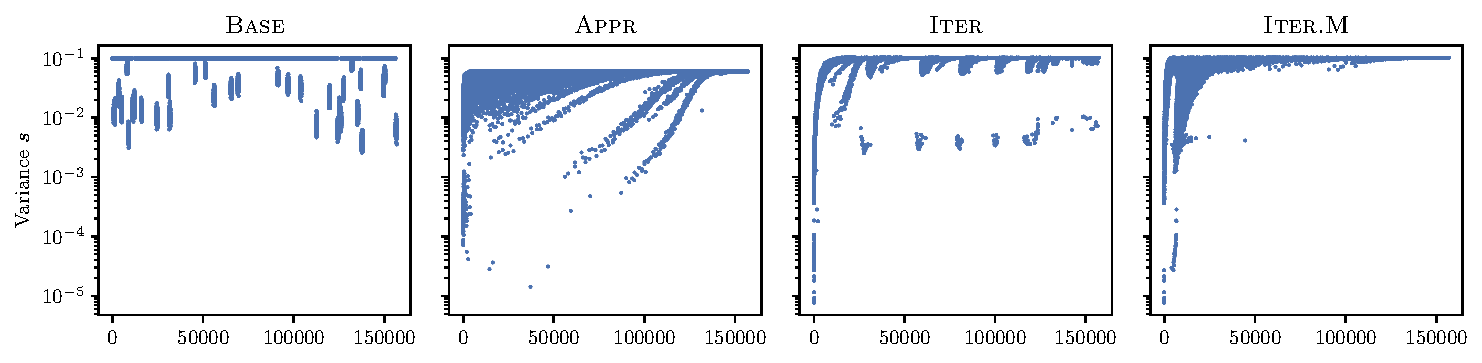
\includegraphics[width=0.9\textwidth]{Figures/PacBayes/FC2_10cls/sigma_post_compare_iter_iterH_Sigma_post_MNIST_Exp1FC2_fixlr0.01_fc1.weight.pdf}%
  
%     %\captionsetup{justification=centering}

%     \caption{Optimized posterior variance $\vs$ using different algorithms (fc1:T-$200^2$ trained on MNIST). The horizontal axis denotes the eigenbasis ordered with decreasing eigenvalues. The abbreviation of algorithms are the same as in \cref{tab:pac}.}
%     \label{fig:PAC}
% \vspace{-0.1in}
% \end{figure*}